\documentclass[12pt,a4paper,twoside]{tesi_upf}
% Guidelines for the project are at https://www.upf.edu/smc/projects/
% Template is from https://www.upf.edu/bibtic/en/guiesiajudes/eines/tesis/dina4.html


\usepackage[utf8]{inputenc}
\usepackage[catalan,english]{babel}
\usepackage[cam,a4,center,frame]{crop}

\usepackage[toc,page]{appendix}

\usepackage{tabularx}

\usepackage{enumitem}
\usepackage{amsmath}
\usepackage{MnSymbol}
\usepackage{wasysym}

\usepackage{hyperref}
\usepackage[capitalise,nameinlink]{cleveref}
% Nice formats for \cref
\crefname{section}{Sect.}{Sect.}
\Crefname{section}{Section}{Sections}
\crefname{figure}{Fig.}{Fig.}
\Crefname{figure}{Figure}{Figures}

% Figures
\usepackage{graphicx}
\graphicspath{ {figures/} }

% Fonts
%\usepackage{garamond}
\usepackage{times}

% Sense headings: no modificar
\pagestyle{plain}

\usepackage{makeidx}
\makeindex

\selectlanguage{english}


\title{Tools for building new MIR datasets}
\subtitle{Master thesis}
\author{Roman Tsukanov}
\thyear{2016}
\department{Department of Information and Communication Technologies}
\supervisor{Dmitry Bogdanov}


\begin{document}

\frontmatter
\maketitle

\cleardoublepage

\section*{\Large Abstract}
Datasets are a very important part of research in the Music Information Retrieval. Unfortunately, some of the most used datasets have issues related to their annotation quality and coverage. We develop tools for building datasets with a goal to fix these issues. Our tools work within the AcousticBrainz project. It already has a significant collection of descriptors extracted from user's music collections.

We try to make dataset creation tools more accessible and flexible by providing multiple ways to create and share datasets. These datasets are then used to generate machine learning models for extracting high-level descriptors like mood and genre. In order to encourage people to build datasets we organize challenges where people can compete by building a dataset for specific classification task. One of the main goals is to make datasets open and easily accessible to encourage their use and improvement. Finally, we provide a way for data consumers to provide feedback on high-level output that they see on the website.

\cleardoublepage

\tableofcontents

\mainmatter

\chapter{Introduction}
\label{sec:introduction}

\section{Motivation}
\label{sec:motivation}

In 2014 Music Technology Group\footnote{\url{http://www.mtg.upf.edu}} at the Universitat Pompeu Fabra and MetaBrainz Foundation\footnote{\url{https://metabrainz.org}} started AcousticBrainz project\footnote{\url{http://acousticbrainz.org}}. Its main goal is to collect acoustic information about music recordings and make it available to the public. Data is contributed by users using a client application. This application extracts low-level information about recordings, and submits it to the server.\footnote{In the context of AcousticBrainz, \emph{low-level} data consists of descriptors extracted from audio signal and \emph{high-level} data is inferred from datasets for low-level data using machine learning techniques.} Low-level information includes descriptors like MFCC, spectral centroid, pitch salience, silence rate; rhythm descriptors like BPM, beat position, onset rate; tonal descriptors like key, scale, HPCP, etc. The low-level information is then used to compute high-level descriptors (genre, mood, etc.) using machine learning models.

One of the big problems is quality of high-level data. Datasets and machine learning models generated from them do not produce good enough results most of the time~\cite{sturm2014simple}. Apart from previous research, this problem became apparent after AcousitcBrainz users started analysing their collections of recordings, which are much more extensive compared to what is available within the Music Information Retrieval (MIR) community \cite{crosscolleval}. Majority of datasets that are currently used for genre classification contain no more than 1,000 recordings. Structure of these datasets is not good enough either. For example, datasets for genre classification contain no more than 10 genre labels in them. Some of the datasets are not publicly accessible to researchers, so it's difficult to review and improve them \cite{porter2015acousticbrainz}. There are very few publicly available datasets for some semantic facets (instrumentation- or culture-related datasets). Classifiers that are currently used in AcousticBrainz, for example, are based on many private in-house collections\footnote{\url{https://acousticbrainz.org/datasets/accuracy}}.

There is no open framework for community-based systematic creation of datasets, evaluation, collection of feedback. MIREX framework, which is overviewed in the next chapter, is a good platform for evaluation of MIR systems and algorithms that encourages advancements in the MIR field. Despite all its issues, it can be a good model for organizing challenges related to dataset creation. The goal of these challenges would be to improve quality of datasets used for a specific classification task: genre recognition, mood classification, instrument detection, etc.

\section{Goals}

The main goal of this project is to provide open framework for dataset creation described in the previous section.

\begin{enumerate}
    \item Provide tools to simplify creation and sharing of MIR datasets for classification tasks.
    \item Encourage people to create, evaluate, improve and share datasets by organizing dataset creation challenges.
    \item Add a way for people to provide feedback on high-level data produced from models.
    \item Improve quality and variety of datasets that are used in the MIR
\end{enumerate}

\chapter{State of the art}
\section{Overview}

This chapter describes current state of things in MIR and other fields related to the project. First, I go through the MIREX framework, giving brief overview of its structure and issues. I also describe some notable datasets that are actively used in the MIR field, how they were built, and what problems they have. In addition to that, I provide some information about how datasets in MIR and other fields are generally created and evaluated. In the end conclusions are made and ideas for work that can be done in this project are outlined.

\section{MIREX}

\subsection{Overview}

Music Information Retrieval Evaluation eXchange (MIREX) is the framework for the formal evaluation of MIR systems and algorithms \cite{downie2008mirex}. It is coordinated and managed by the International Music Information Retrieval Systems Evaluation Laboratory\footnote{\url{http://music-ir.org/}} (IMIRSEL) at the University of Illinois at Urbana-Champaign\footnote{\url{http://illinois.edu/}}.

MIREX is a direct descendant of ``Audio Description Contest'', which was convened by the Music Technology Group (MTG) at Universitat Pompeu Fabra in 2004 \cite{ismir2004description}. Both were inspired by Text Retrieval Conference (TREC) framework \cite{voorhees2005}.

All these frameworks try to standardise tasks that are performed on test collections of significant size and evaluation methods used to assess the quality of results. In case of MIREX, set of tasks and evaluation methods is largely determined by the community discussion. After community and organizers settle on what tasks they want to have as a part of next MIREX challenge, evaluations are run in July and August. Results are presented at the International Society of Music Information Retrieval (ISMIR) conference. The whole process takes about a year.

\subsection{Evaluation process}

One significant difference between TREC and MIREX is that datasets for each task are not freely distributed to the participants. All the data is stored in one central location at IMIRSEL. There are several reasons for this. Two most important are:
\begin{enumerate}
    \item Avoiding the possibility of participants to tune their algorithms specifically for the dataset.
    \item Current state of intellectual property copyright enforcement.
\end{enumerate}
Second reason generally affects MIR research in a negative way, making it harder to collect music datasets and experiment with them.

The way MIREX challenge works then is by gathering algorithms from all the participants and running them on organizer's infrastructure. All this introduces several significant challenges:
\begin{enumerate}
    \item A lot of time is spent finding, obtaining, and managing data for evaluation.
    \item Creating ground-truth data of a good quality takes a lot of resources.
    \item There is a high chance of having errors in annotations of ground-truth data and test collections.
    \item Algorithm-to-data model causes issues with capacity. Apart from terabytes of raw audio data, some algorithms that are run on this data require significant amount of intermediary storage.
    \item It takes a lot of time to manage submitted algorithms.
\end{enumerate}

According to the MIREX overview paper \cite{downie2008mirex}, there are several key issues that need to be addressed:
\begin{enumerate}
    \item Resource accessibility (music collections, ground-truth sets, pre-built models, etc.).
    \item Discovery tools for resources.
    \item Sharing and re-use of resources.
    \item Resource customization and integration.
\end{enumerate}

\section{Datasets}
\label{sec:soa:datasets}

\subsection{Overview}

\begin{table}[h]
    \footnotesize
    \centering
    \begin{tabular}{l|l|l}
        Name & Type & Size \\
        \hline
        GTZAN & Genre & 1,000 items (10 labels) \\
        ISMIR2004 Tempo Classification Dataset & Ballroom music styles & 698 items (8 labels) \\
        Music Audio Benchmark Dataset (Dortmund) & Genre & 1,886 items (9 labels) \\
        MIREX Audio Mood Classification Dataset & Mood & 1,250 items (5 clusters) \\
        MagnaTagATune & Similarity & 25,863 items (30s) \\
        The Million Song Dataset & Metadata and audio features & 1,000,000 items \\
    \end{tabular}
    \caption{Notable datasets used in MIR}
    \label{tab:mirdatasets}
\end{table}

\subsubsection{GTZAN}

GTZAN \cite{tzanetakis2002} is a dataset for music genre recognition (MGR) research, created in 2002. It has several problems: repetitions, mislabelings, and distortions \cite{sturm2013gtzan}. It is created by one person, which produces bias. It's not very diverse: many tracks are by the same artist and/or from the same album. Other major fault that is often pointed out is its size. It contains 1,000 excerpts, which is much less compared to some personal music collections (thousands of recordings) or commercial datasets and library archives (millions of recordings). It is also significantly outdated. Despite all these problems it is still one of the most actively used datasets in MGR.

\subsubsection{ISMIR2004 Tempo Classification Dataset}

ISMIR2004 Tempo Classification Dataset \cite{ballroom} was a part of audio description contest at ISMIR 2004\footnote{\url{http://ismir2004.ismir.net/ISMIR_Contest.html}}. It consists of 698 excerpts of a ballroom dance music and was meant to be used for tempo (BPM) induction. The music itself was collected from the website \href{http://www.ballroomdancers.com}{BallroomDancers.com}.

\subsubsection{Music Audio Benchmark Dataset}

Music Audio Benchmark Dataset\footnote{\url{http://www-ai.cs.uni-dortmund.de/audio.html}} \cite{dortmund} (also known as ``Dortmund'' dataset) is a dataset for genre classification. It consists of 10 seconds samples (drawn from a random position) of 1,886 songs which were obtained from the Garageband.com website. It contains 9 genre labels and additional metadata. Metadata includes information like total length, name of the band or artist, information about genre, user comments, and lyrics (partially). In addition, it provides 24 cluster models created manually by a group of users using arbitrary personal viewpoints.

This dataset also contains additional classification schemes created by users. They vary in size and cover different subsets of songs. Users classified songs according to aspects like genre, quality, preference, time of day, instruments, singer, etc.

\subsubsection{MIREX Audio Mood Classification Dataset}

MIREX Audio Mood Classification Dataset \cite{hu2007exploring,hu2008} was created to serve the need of automated classification of mood in music recordings. It was derived from metadata from AllMusicGuide.com website which, at the time, provided reviews and metadata for artists, albums, and songs. 

It consists of 5 mood clusters, each containing some specific ``mood spaces''. For example, one of the clusters contains the following ``mood spaces'': visceral, volatile, fiery, aggressive, tense/anxious, intense.

Tracks for this dataset were selected from the Associated Production Music (APM)\footnote{\url{http://www.apmmusic.com/}} collection, which is available to the MIR community under a contract of academic use between APM and IMIRSEL. From original collection of 206,851 tracks 1250 were selected (250 in each cluster). Each track there is annotated with various metadata fields like category (mood and other descriptors), instrumentation, tempo, style, and others. Selection was done by applying a number of filtering steps:
\begin{enumerate}
    \item Removal of tracks without genre information to be able to explicitly select tracks from different genres.
    \item Matching mood-related descriptors to specific clusters.
    \item Removal of tracks shorter than 50 seconds to avoid inclusion of non-music content.
    \item Removal of tracks from the same CDs to improve variety.
\end{enumerate}

In addition to original dataset, ground-truth set of 600 tracks was created. Labeling was done by people using a web service designed for MIREX evaluations - Evalutron 6000 \cite{gruzd2007evalutron}. People were instructed to ignore lyrics, since music processing technology was not sufficiently developed to transcribe them and use for classification. They were also trained on a set of examples for each mood cluster. If none of the clusters were appropriate, people could select category ``Other''. In the ground-truth set only tracks with at least two agreed labelings were used.

\subsubsection{MagnaTagATune}

MagnaTagATune\footnote{\url{http://mirg.city.ac.uk/codeapps/the-magnatagatune-dataset}} \cite{magnatagatune} was created using TagATune game \cite{tagatune} and music from the Magnatune label\footnote{\url{https://magnatune.com/}}. It contains 25,863 audio clips from 5,405 source MP3s. Each clip is assigned tags by users of TagATune. In addition, it contains a detailed analysis of the structure and musical content (rhythm, pitch, timbre) from The Echo Nest\footnote{\url{http://the.echonest.com/}}.

\subsubsection{The Million Song Dataset}

The Million Song Dataset \cite{millionsongdataset} provides large-scale dataset to MIR researchers. Larger datasets are hard to build because of licencing issues and Million Song Dataset's aim is to solve this problem. It doesn't include audio, only features extracted from it and additional metadata. Features were extracted from The Echo Nest Analyze API and are mainly \textit{pitches}, \textit{timbre}, and \textit{loudness}.

The Million Song Dataset is also a cluster of complementary datasets contributed by the community\footnote{\url{http://labrosa.ee.columbia.edu/millionsong/pages/additional-datasets}}:
\begin{itemize}
    \item SecondHandSongs dataset (cover songs)
    \item musiXmatch dataset (lyrics)
    \item Last.fm dataset (song-level tags and similarity)
    \item Taste Profile subset (user data)
    \item thisismyjam-to-MSD mapping (user data)
    \item tagtraum genre annotations (genre labels)
    \item Top MAGD dataset (genre labels)
\end{itemize}

That dataset has a couple of problems:
\begin{enumerate}
    \item It's not being updated, so fixes for problems aren't available to everyone.
    \item Computed descriptors are based on closed algorithms, which means that it's difficult to review them.
\end{enumerate}

\subsection{Creation}

Most datasets that I went though are created based on annotations by humans. Some use tags or other information scraped from websites like Last.fm. Some use a dedicated tool for manual tagging like TagATune or Evalutron 6000. Quality of datasets created from tags is directly related to correctness of these tags.

Most of Last.fm tags, for example, are related to different styles of music, genres. These are often used to generate genre datasets. Genre is a subjective thing so it's important to make sure that items which are being included in a dataset have tags that are agreed upon by majority of users. In case of Last.fm it is possible to see how many users have assigned the same tag to a recording. Some other services have similar functionality.

GTZAN is created by one person, which introduces bias into contents of that datasets. This can be avoided using collaborative creation process.

\subsubsection{In other domains}

\begin{figure}[!htb]
  \centering
  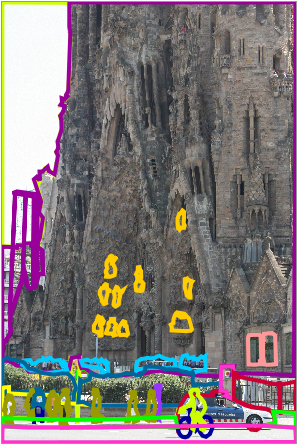
\includegraphics[width=0.80\textwidth]{labelme}
    \caption{LabelMe annotation example \textit{(taken from \url{http://labelme2.csail.mit.edu/})}}
    \label{fig:labelme}
\end{figure}

\begin{figure}[!htb]
  \centering
  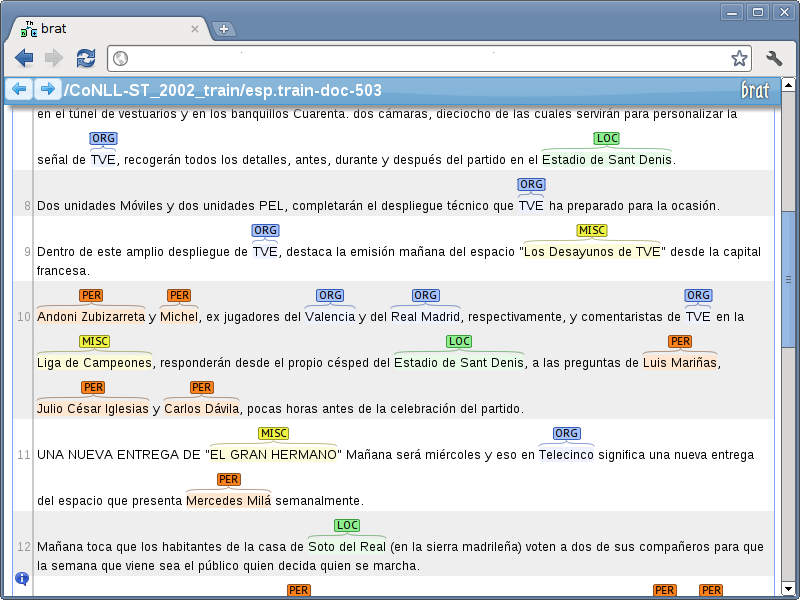
\includegraphics[width=0.80\textwidth]{brat}
    \caption{BRAT \textit{(taken from \url{http://brat.nlplab.org})}}
    \label{fig:brat}
\end{figure}

Similar tools for dataset creation exist in other domains. One example is an image annotation tool called \textbf{LabelMe}\footnote{\url{http://labelme2.csail.mit.edu/}} \cite{labelme} (see figure \ref{fig:labelme}). It is used in object detection and recognition research. Creation of ground-truth data is done through the website. Users upload images and annotate different parts of them by assigning labels like ``tree'', ``window'', ``person'', or some other.

Another is \textbf{brat rapid annotation tool (BRAT)}\footnote{\url{http://brat.nlplab.org}} -- a web-based tool for text annotation, used in natural language processing (NLP) field \cite{brat} (see figure \ref{fig:brat}). It attempts to provide an intuitive and user-friendly with a goal of making annotation more accessible to non-technical users and improving annotation productivity.

\subsection{Evaluation}

Sturm in \cite{sturmfuture} makes several suggestions for improving scientific research in MIR, including some related to evaluation and analysis of results:
\begin{itemize}
    \item Analysis that answers a question of how well the ground-truth of a dataset is shallow and has limited use. This kind of analysis doesn't provide knowledge how the system is operating or whether its performance is satisfactory for a particular use case. The aim should be to produce knowledge, not publication arising from statistical significance.
    \item Acknowledge limitations that all experiments have when drawing any conclusions from them, and to be suspicious of results because some of them seem too good to be true.
    \item Make the work reproducible. It's important to publish and make accessible enough code and resources that were used for evaluation, testing, and other stages of work. Though sometimes, even when this is done, there are errors or other issues that cause the system to produce different results.
\end{itemize}
He also analyzed methods that are used during evaluation (focused on MGR) and showed that ``classification accuracy is not enough'' \cite{sturm2013}.

\section{AcousticBrainz}
\label{sec:soa:acousitcbrainz}

\subsection{Project summary}

As described in section~\ref{sec:motivation}, AcousticBrainz project collects acoustic information which is extracted from users' music collections using the client application \cite{porter2015acousticbrainz}. At the moment of writing it contained more than 2.2 million unique and 4.1 million total submissions from the community.

\subsection{Audio descriptors}

When users run AcousticBrainz client on their audio files, it extracts a set of \textbf{low-level descriptors} using Essentia library \cite{essentia}. Low-level data includes acoustic descriptors which characterize overall loudness, dynamics and spectral shape of a signal, rhythm descriptors, and tonal information.

In addition to low-level descriptors, client submits metadata about a recording:
\begin{itemize}
    \item Codec information and sampling rate
    \item Length of a recording
    \item Version of extractor
    \item Recording name and its \textbf{MusicBrainz Identifier (MBID)}\footnote{\url{https://musicbrainz.org/doc/MusicBrainz_Identifier}}
    \item Artist name and their MBID
    \item ...and other information that is stored in file's tags.
\end{itemize}
Recording MBID might be the most important piece of metadata. All user submissions are recordings that need to be tagged with an MBID. This can be done with one of taggers like MusicBrainz Picard\footnote{\url{https://picard.musicbrainz.org/}}. MBIDs are permanent identifiers that allow to lookup data on MusicBrainz and other projects that support them.

Based on low-level data AcousticBrainz server computes a number of \textbf{high-level descriptors} from low-level data using machine learning models. These are descriptors like timbre, gender, mood, genre, etc.

\section{Conclusions}

\subsection{MIREX}

MIREX is a great framework that encourages advancements in the MIR field by providing a broad set of evaluation tasks\footnote{\url{http://www.music-ir.org/mirex/wiki/2016:Main_Page#MIREX_2016_Possible_Evaluation_Tasks}}. Unfortunately, it's not very flexible to have only one set of challenges per year. This makes it hard to quickly iterate on results, which significantly slows down the research process. Having a framework that can automate or simplify common tasks that are done to prepare such challenge can be very beneficial for the MIR community.

As pointed out in the overview paper \cite{downie2008mirex}, it is difficult to acquire, validate, and store test collections and ground-truth data, which is essential for development of MIR systems. The biggest reason is the current state of copyright in the music industry. There needs to be an easy way to store and share datasets with other researchers.

\subsection{Datasets}

\subsubsection{Creation}

Datasets that are currently used in MIR have a number of problems. These, of course, don't apply to every dataset out there, but most do have some of them.
\begin{itemize}
    \item Size is too small to get good results using machine learning algorithms.
    \item Outdated and don't include new recordings.
    \item Mislabelings, repetitions, bias and other issues with content.
\end{itemize}

As motivation for creation of The Million Song Dataset \cite{millionsongdataset} describes, there are several advantages to creating a large dataset:
\begin{itemize}
    \item It helps reveal problems with scaling of algorithms, which is critical for ``real-world'' use.
    \item Some phenomena or patterns might not be discernible in a small dataset.
    \item It can be more comprehensive, include more specific subsets.
    \item When freely-available, directly promotes comparison of usage results and interchange of ideas.
\end{itemize}

Significant number of datasets are based on crowd-sourced annotations from services like Last.fm\footnote{\url{https://www.last.fm/}} and beaTunes\footnote{\url{https://www.beatunes.com/}} \cite{schreiber2015}. MusicBrainz -- a popular music encyclopedia -- allows editors to assign tags to different entities in the database\footnote{\url{https://musicbrainz.org/doc/MusicBrainz_Entity}}. Most of these services allow users to vote on tags or submit already existing tags. This information can be used to determine which tags are more agreed upon than others, and to automate generation of datasets.

Creation of datasets should be a simple process. As mentioned before, tools for annotation (labeling) exist in other domains. These tools simplify annotation which ultimately improves quality of datasets produced from them. Some lessons can be learned from how they work and be applied to MIR research. While we already have datasets based on annotations from services like Last.fm, it can be useful to streamline this process of generating datasets from different sources.

Simplicity is also important in cases when users have to work with these datasets. This includes tasks like organizing contents and making sure that structure is correct, exporting datasets to perform analysis in some other tools, importing datasets that were created externally into a central repository (AcousticBrainz).

Bias in the process of creation of datasets can be avoided by allowing people to work collaboratively and by integrating user feedback from results of evaluation.


\chapter{Methodology}
We take the following approach:
\begin{enumerate}
    \item Implement a platform for creating and sharing datasets
    \item Implement a way to build machine learning models based on datasets
    \item Organize dataset creation challenges
    \item Provide a way to get feedback from users
\end{enumerate}

\emph{The focus will be on datasets and their structure instead of algorithms.}

%%%%%%

\section{Dataset creation and sharing}

As described in the motivation, datasets are important part of MIR systems. Some of the datasets that are currently used have issues with the way they are built. Sometimes it's hard to reproduce results because it's unclear which specific recording is used. Sometimes datasets disappear from official sources and become difficult to find.

In this project the idea is to have a centralized directory of datasets which people can use to store their datasets, find datasets created by other members of the community and use them. In addition to storing datasets, we also provide a way to create datasets.

Dataset creation can be implemented in several ways:
\begin{itemize}
    \item Importing datasets created externally using user tagging tools, scraping data from various websites, etc.
    \item Manual creation using a web-interface
    \item Automated generation of datasets using labels, assigned to recordings by users
\end{itemize}

Structure of each dataset is simply a set of named classes with recordings in them. We'll require to use permanent identifiers (MBIDs) to reference recordings. This will solve an important issue of identifying items in a dataset. Many existing datasets are based on unknown audio excerpts or other types if items which don't have any useful identifiers. This means that it's impossible to reconstruct such datasets and reproduce work that's been done before. And there is no way to map them to other datasets. In AcousticBrainz each low-level submission is associated with an entity in MusicBrainz database using an MBID.

Each dataset will be assigned a unique identifier and listed on the website. Everyone will be able to browse and download it for further use.

The whole dataset creation system doesn't necessarily need to be closely tied to AcousticBrainz. Everyone should be able to retrieve datasets and use them in any other project with other tools. One of the most important aspects of the AcousticBrainz project is that all data is open. We believe that this open policy helps community share new ideas and advancements.

%%%%%%

\section{Building machine learning models}

After a dataset is created, it can be used to train a machine learning model for extracting high-level data. AcousticBrainz project doesn't have direct access to audio files after they are analyzed by a client software\footnote{\url{https://acousticbrainz.org/download}}, only a set of low-level descriptors that were extracted by the Essentia library embedded in a client. These descriptors, however, can still be used with the \textit{Music extractor} of the Essentia library\footnote{\url{http://essentia.upf.edu/documentation/streaming_extractor_music.html}}.

It's important to make the work reproducible, so we share all the code that is written for the project. All of the components used in the AcousticBrainz project are open-source, including web server for collecting data, extractor, and software for evaluation of that data.

%%%%%%

\section{Dataset creation challenges}

\subsection{Overview}

One way to encourage people to build datasets for specific classification tasks is to organize challenges with a goal to build datasets that result in an accurate model for extracting high-level data. It's important that participants are able to iterate on results quickly using tools that we provide to them. MIREX challenges are conducted annually, which slows down improvements. We'd like to speed up this cycle.

A significant difference from MIREX would be that we are focusing on datasets for \emph{classification} tasks, not underlying algorithms that do feature extraction from audio files and train classifiers.

Everyone will be allowed to participate. We hope that simplifying the tools and making the process open will be very beneficial for the MIR community.

\subsection{Potential issues}

There are a couple of issues that needs to be considered during the implementation of dataset creation challenges:

\begin{enumerate}
    \item There needs to be an independent dataset that will be used to measure accuracy of all models generated from submissions. This dataset can be created by the organizer.
    \item Datasets that are submitted for a challenge need to be hidden from the public until the challenge ends. Otherwise anyone would be able to use pretty much the same dataset that other person submitted, make slight changes and get higher accuracy as a result. That would result in an unfair competition.
\end{enumerate}

\subsubsection{Cross-validation with an independent dataset}

\emph{This is probably the most important issue that needs to be solved to make a more reliable system for conducting the challenges.} Having a separate dataset, that is used to cross-validate all datasets submitted by users, is essential to make sure that all submissions can be measured against each other. Otherwise, someone can come up with a dataset that would have a model which will have a 100\% accuracy during training and win a challenge. The problem is that dataset will be highly overfitted and useless for any real-world application.

A solution is to make model training from datasets submitted for a challenge a two step process:
\begin{enumerate}
    \item Training a model based only on contents of the dataset.
    \item Applying model to an independent dataset and measuring resulting accuracy.
\end{enumerate}

Cross-validation dataset can be created by organizers of a challenge. Ideally, multiple people should be able to collaborate on creation of this kind of dataset. After each dataset goes through the training process and produces a best working model, that model is tested on cross-validation dataset and results are compared with other datasets. Testing means comparing if class label that each recording is assigned matches expected value that is defined in cross-validation dataset.

Structure of that independent dataset (set of classes used in it) needs to be the same as in all submissions. It's also important that definitions of classes (labeling) for each recording is correct, so that challenge participants can trust results of accuracy measurements based on it. In order to gain that trust, validation dataset should be made public. This, however, introduces another constraint for creation process: all datasets created for a challenge will need to have recordings filtered so that they don't match ones in the validation dataset. Otherwise this might open ways to cheat the evaluation system.

\subsubsection{Dataset privacy}

Another important thing to do, to be able to conduct fair challenges, is to hide contents of datasets submitted for a challenge. Otherwise, anyone can replicate the result by making slight modifications to the original dataset that would be enough to increase accuracy and submit it for the same challenge. This would create an unfair competition for participants.

Contents of all submissions can be hidden until the end of submission process. After that it is important to publish all of the submissions, so that other people can reproduce the results and do further improvements. The last part is essential, as one of the main goals of AcousticBrainz project is to keep all the data public.

%%%%%%

\section{User feedback}

In order to improve quality of a model and underlying dataset there needs to be a way to do meaningful iterations on them. User feedback can help find errors in the output that the model produces. It can also be an additional way to populate dataset with more items. Users can give their opinion on whether the output is right or wrong. And, possibly, which \textit{class} recording should be in if it has not been classified correctly. Set of classes that will be presented to a user can be obtained from a version of the dataset that was used to train the model. There might be an option for user to say that recording doesn't belong in any of the existing classes and suggest some other one.

Feedback submitted by users can be used by dataset author or other creators to improve contents of datasets related to a specific classification problem (genre, mood, etc.). They can include recordings that received significant number of votes into a dataset to make it more comprehensive.

This feedback can also be used to measure overall performance of a model. We can decide which ones to keep \emph{active}\footnote{Active models are used to calculate high-level data from all submissions.} and which ones need to be deactivated or replaced with some that might perform better.


\chapter{Implementation}
\section{Introduction}

% TODO: Review the list below
This chapter describes implementation details of different components of the project. All of these components are part of the AcousticBrainz Server\footnote{\url{https://github.com/metabrainz/acousticbrainz-server}}:
\begin{itemize}
    \item Dataset creation
    \item Model training
    \item Challenge management interface
    \item Dataset submission process and different stages of a challenge
    \item Evaluation of results
\end{itemize}

%%%%%%

\section{Dataset creation}

\subsection{Overview}

To cover most basic use cases we have three ways to create a dataset:
\begin{itemize}
    \item Web-based editor
    \item Importer from CSV file
    \item Web API
\end{itemize}

The overview of how datasets are processed and used in the projects is shown in figure \ref{fig:dataset_creation}.

\begin{figure}[h]
  \centering
  \includegraphics[width=0.80\textwidth]{dataset_creation}
    \caption{Overview of the dataset lifetime in the AcousticBrainz project}
    \label{fig:dataset_creation}
\end{figure}

\subsection{Web-based editor}

The easiest way for people to start building a dataset is to use an editor that is integrated with the AcousticBrainz website. It doesn't require user to have any additional tools.

Editor interface is implemented using a JavaScript framework called ``React''\footnote{\url{https://facebook.github.io/react/}}. It allowed us to build an interface that is easy and fast to use. Behind the scenes, it relies on the web API of AcousticBrainz Server which provides endpoints for editing datasets. Same API can be used by people to create datasets directly using their own tools. We think it's a good idea to use the same interface that is available to the rest of users. That way we can make sure that it is as complete as possible. It is also a good software engineering practice to have a multitier architecture\footnote{\url{https://en.wikipedia.org/wiki/Multitier_architecture}}.

\begin{figure}[h]
  \centering
  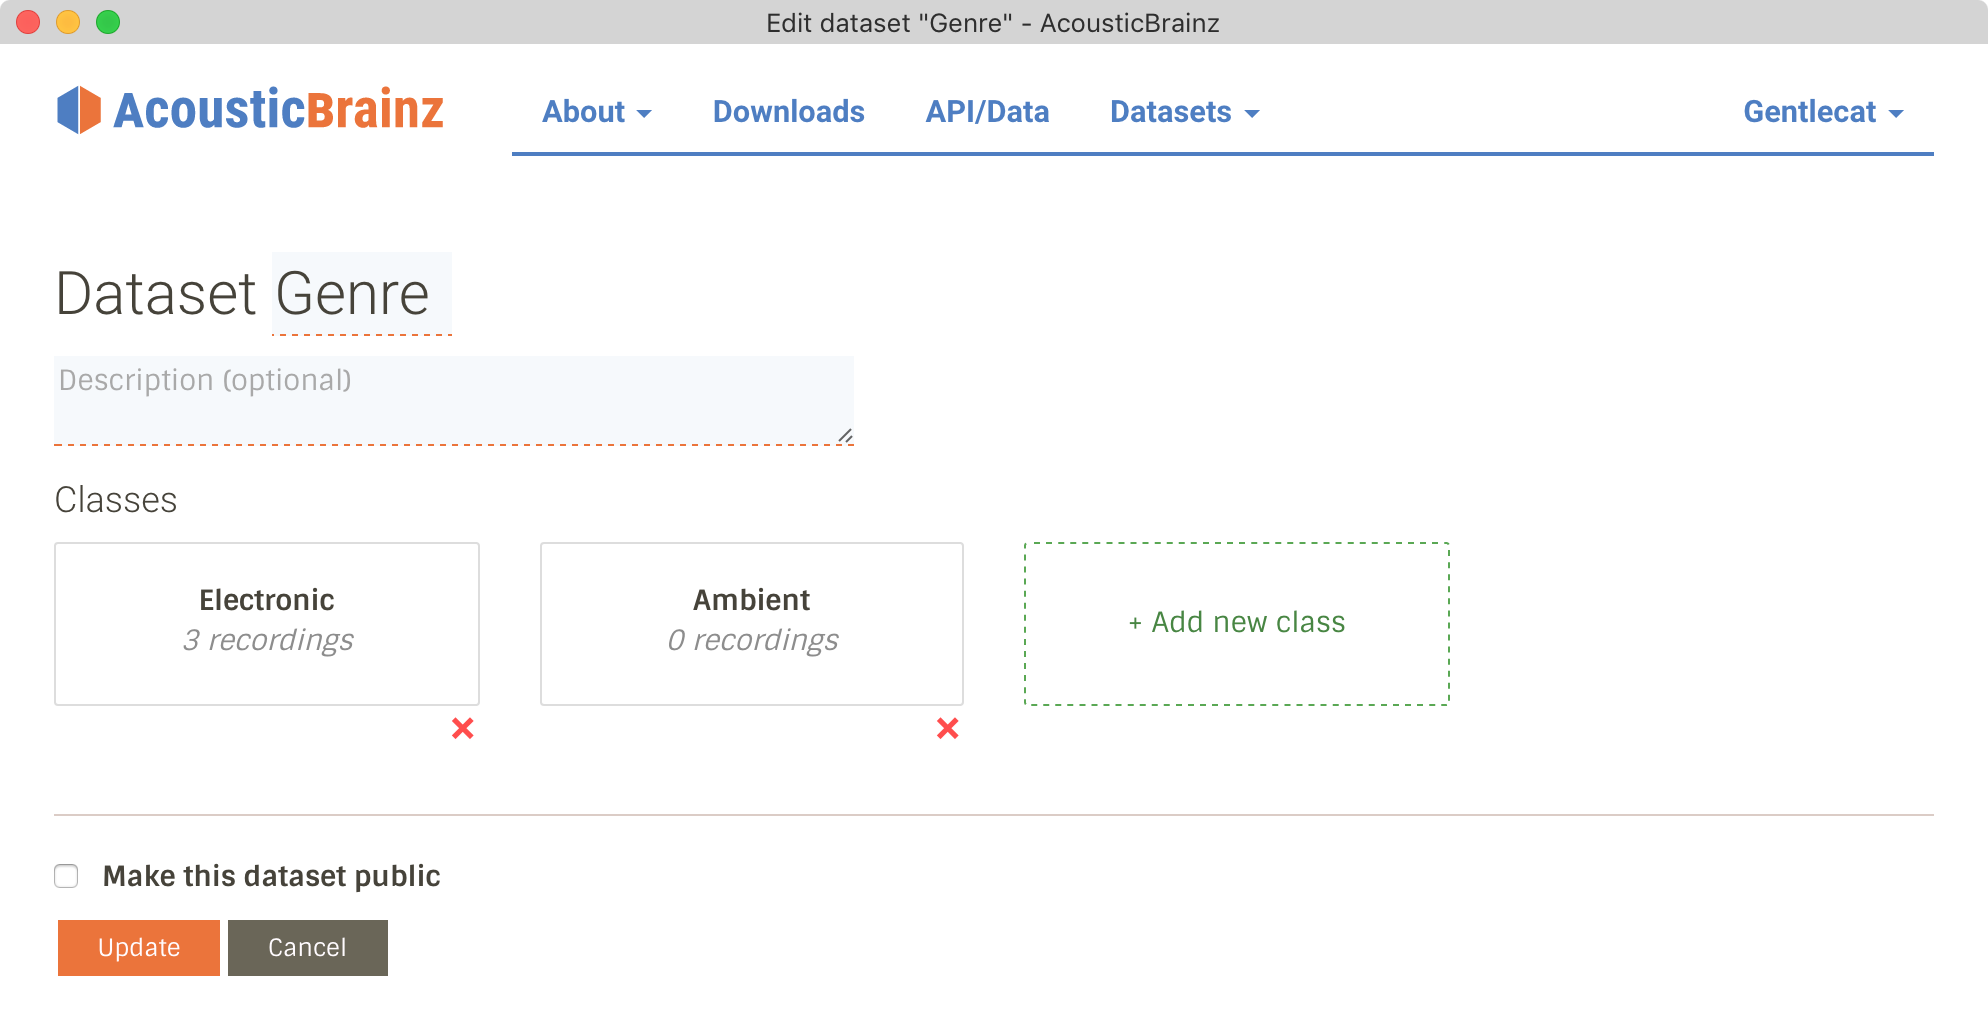
\includegraphics[width=\textwidth]{editor_overview}
    \caption{Main page of the dataset editor}
    \label{fig:editor_overview}
\end{figure}

Figure \ref{fig:dataset_creation} shows the main view of the dataset editor. Here user can do the most basic things like naming a dataset, describing it, defining its structure by specifying a set of classes. From that view users can access each individual class.

\begin{figure}[h]
  \centering
  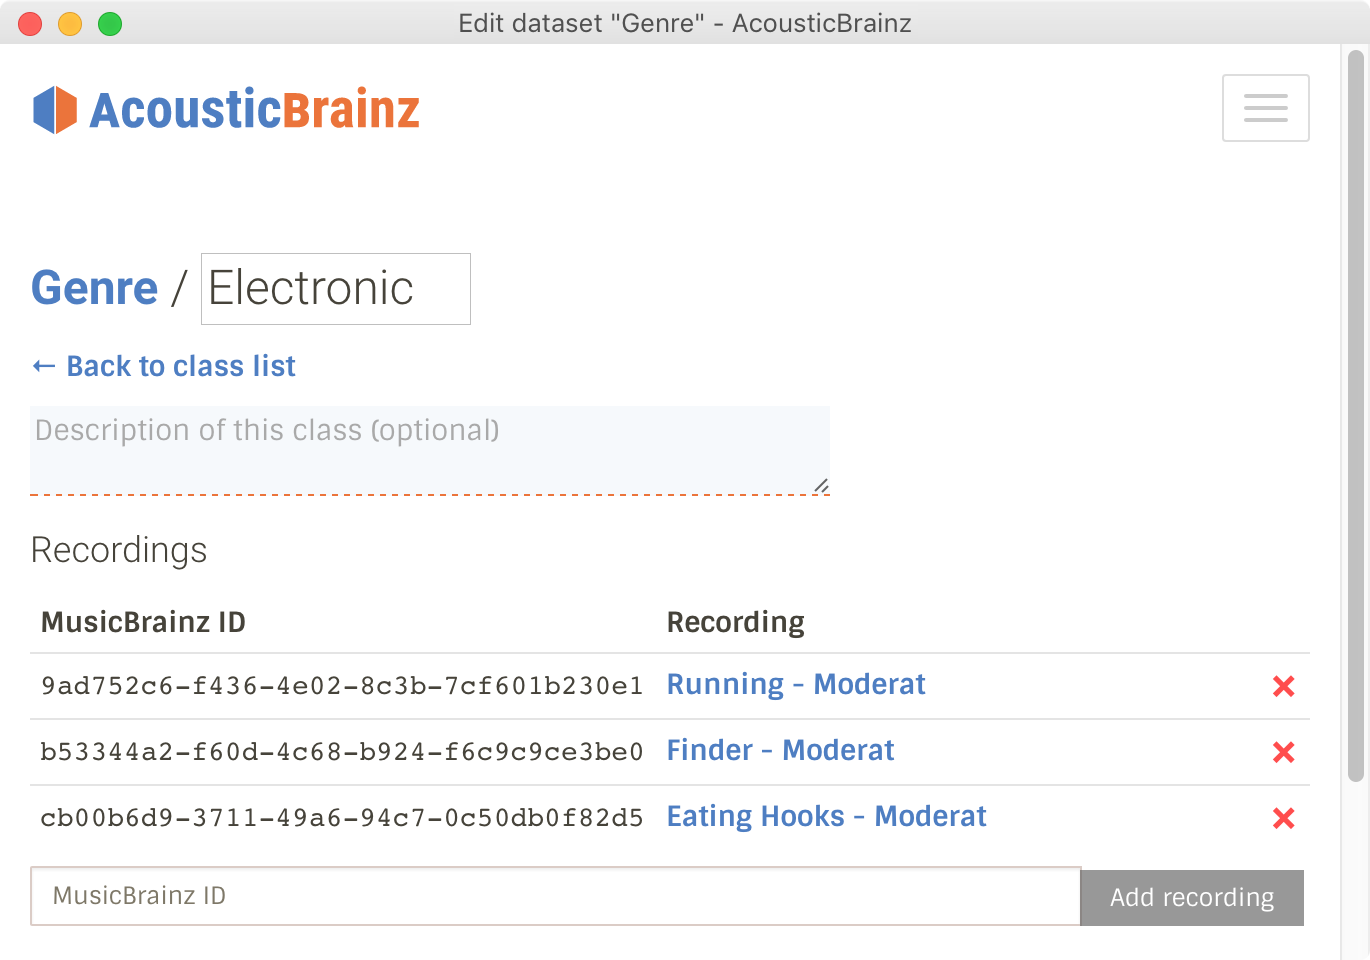
\includegraphics[width=\textwidth]{editor_class}
    \caption{Class view in the dataset editor}
    \label{fig:editor_class}
\end{figure}

In the class view (figure \ref{fig:editor_class}) it's possible to modify recordings\footnote{\url{https://musicbrainz.org/doc/Recording}} that each class contains. All recordings are referenced by MBIDs. For each recording we load its name and name of the associated artist(s) from the MusicBrainz Web Service.

When user is done editing a dataset they can save the changes.

\subsection{CSV importing}

Some researches have their own tools that they work with and, specifically, build and analyze datasets: MATLAB, Python, etc. We think that it would be useful to add a simple way for the to get started using new features in AcousitcBrainz project by importing their datasets in CSV format\footnote{\url{https://tools.ietf.org/html/rfc4180}}.

Supported CSV files must have the following structure: \textit{\textless MusicBrainz Identifier of a recording\textgreater, \textless Class label\textgreater}. Each row in the file defines an ID of a recording and associated class label. After CSV file is ready for import, it can be uploaded to AcousticBrainz where it will be parsed, converted and stored for further use.

\subsection{Web API}

The last way of working with datasets we have is using a web API\footnote{Application Programming Interface, \url{https://en.wikipedia.org/wiki/Web_API}}. It allows users to create and edit datasets by sending HTTP\footnote{\url{http://httpwg.org/specs/}} requests to AcousticBrainz server.

API has the following endpoints:
\begin{itemize}
    \item Create a dataset
    \item Retrieve a dataset
    \item Update details (name, description) of a dataset
    \item Delete a dataset
    \item Add class to a dataset
    \item Update class in a dataset (name, description)
    \item Remove class from a dataset
    \item Add recordings into a class
    \item Remove recordings from a class
\end{itemize}

\textit{All of these endpoints are described in more detail in AcousticBrainz documentation\footnote{\url{https://acousticbrainz.readthedocs.io/api.html\#datasets}}.} It is a useful addition to existing ways to create a dataset, which can encourage users to make their own tools that can help with the creation process.

\subsubsection{Authentication}

Authentication is done using API keys that need to be passed with every request. In order to obtain an API key, users need to login into their AcousticBrainz profile and click ``Generate new key'' button (see figure \ref{fig:api_key}).

\begin{figure}[h]
  \centering
  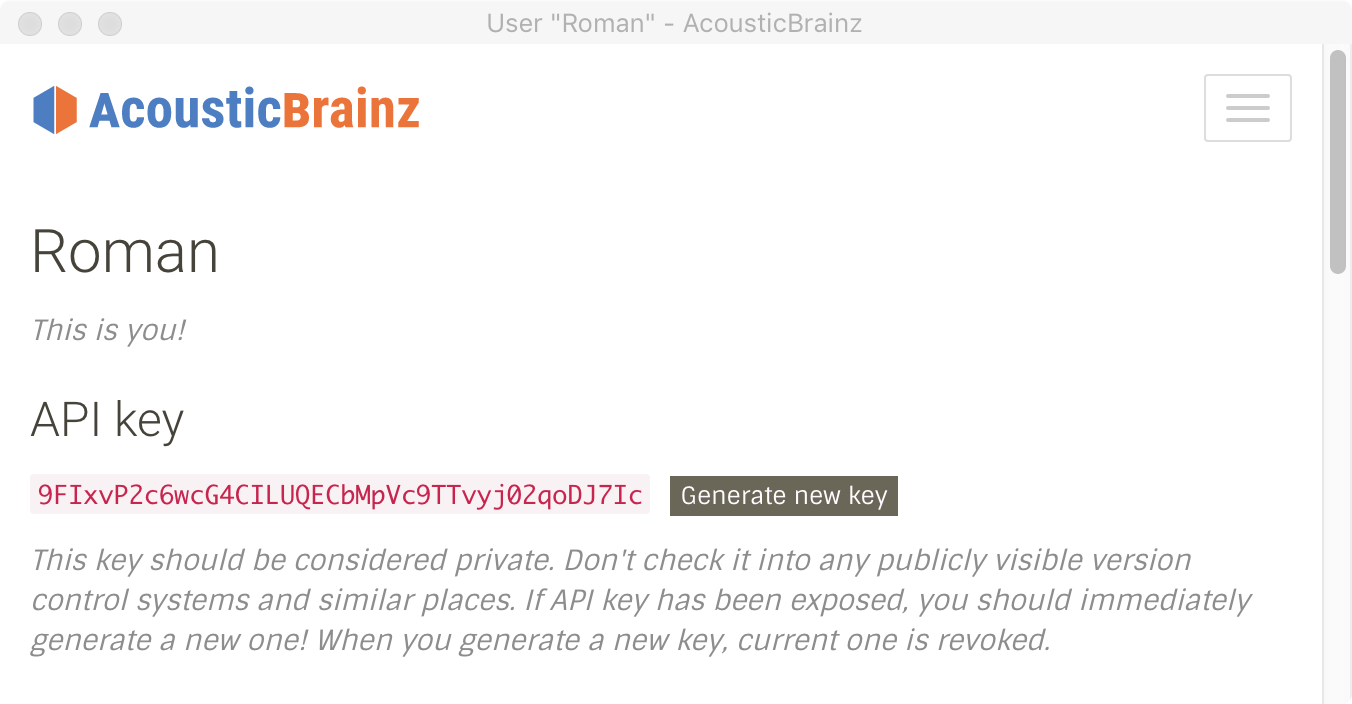
\includegraphics[width=0.80\textwidth]{api_key}
    \caption{Profile page with API key generator}
    \label{fig:api_key}
\end{figure}

API key is randomly generated from lowercase and uppercase ASCII\footnote{American Standard Code for Information Interchange, \url{https://en.wikipedia.org/wiki/ASCII}} letters and digits. Its length is always 40 characters. Currently, only one API key per user account is allowed.

All keys are meant to be kept private. Person who has access to a specific API key can perform actions on behalf on the owner of that key. In case the key is exposed, it is possible (and highly recommended) to generate a new one.

The key privacy limitation means that some uses can become more complicated. For example, in order to build a web application on top of AcousticBrainz API there will need to be a back-end server that would store the API key and attach it to all requests to AcousticBrainz. This, however, shouldn't be a factor when only one person is using a key.

\cite{farrell2009api} describes how API keys are typically used with web APIs, some of the issues involved, and ways to improve. He recommends to use OAuth protocol\footnote{\url{http://oauth.net/}} as a better alternative. This can be one of the future improvements that we make in AcousticBrainz.

%%%%%%

\section{Challenges}

\subsection{Challenge lifetime}

From start to finish each challenge is composed of the following steps:
\begin{enumerate}
    \item Organizer creates a challenge.
    \item Challenge begins and participants submit their datasets.
    \item Submission period ends.
    \item Challenge concludes after results are calculated.
\end{enumerate}

\begin{figure}[h]
  \centering
  \includegraphics[width=\textwidth]{challenge}
    \caption{Overview of the challenge process}
    \label{fig:challenge}
\end{figure}

\subsubsection{Creation of a challenge}

When organizer creates a challenge, they need to define its name, set of classes that are required to be in a dataset, reference to validation dataset that will be used to measure accuracy of submissions, and a time period in which submissions are going to be accepted. After creation, each challenge is assigned a UUID\footnote{Universally Unique IDentifier, \url{https://tools.ietf.org/html/rfc4122}}, which is used to reference it throughout the project.

Set of required classes is used to define a ``namespace'' that all submissions must follow. All of the classes must be present in a submission, additional classes aren't allowed. Same requirements apply to the validation dataset, which is checked during creation.

Interface for creating (see figure \ref{fig:create_challenge}) a challenge is currently available only in the ``admin'' interface, which is accessible to several trusted users. In the future, if needed, challenge creation tools could be made available to all users of AcousticBrainz project.

\begin{figure}[h]
  \centering
  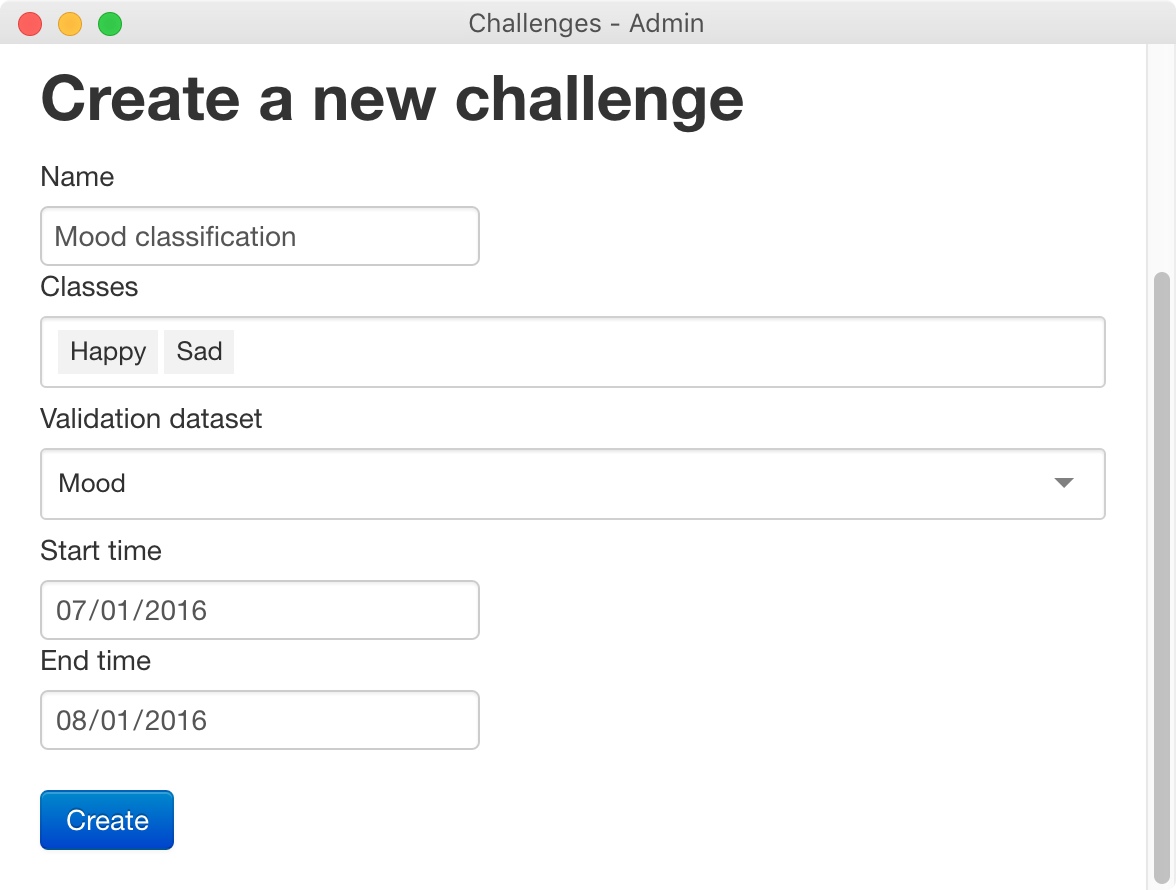
\includegraphics[width=0.80\textwidth]{create_challenge}
    \caption{Challenge creation interface}
    \label{fig:create_challenge}
\end{figure}

\subsubsection{Accepting submissions}

Participation in challenges is open to every user of AcousticBrainz. After creating a dataset with required structure using existing tools, they can submit it for model training as a part of a challenge.

\begin{figure}[h]
  \centering
  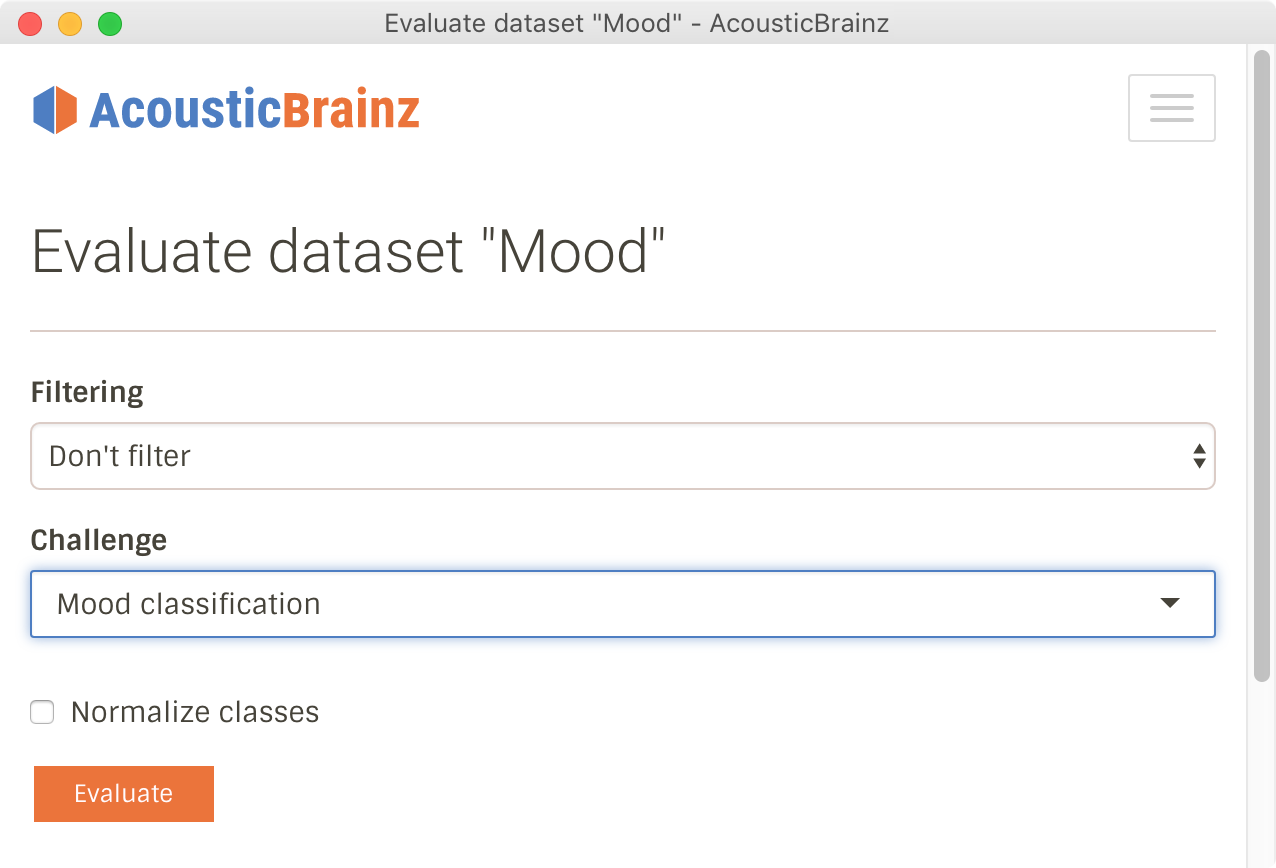
\includegraphics[width=0.80\textwidth]{eval_submission}
    \caption{Training submission interface}
    \label{fig:eval_submission}
\end{figure}

When dataset is submitted, new model training job is added into the queue. In addition to that, dataset structure (list of classes) is checked to make sure that it matches requirements of a challenge. Recording filtering is applied to it (described further).

\subsubsection{Snapshots of datasets}

When user adds dataset into the training queue, regardless of whether it is submitted for a challenge or not, a new snapshot is created. Snapshot of a dataset captures its exact structure at a point of creation: all classes and recordings in them. Snapshots are used to ensure that dataset submitted for model training has a fixed state while it's waiting in the queue or after model is trained. This helps ensure that results (high-level models) are reproducible.

All snapshots are public by default unless they are a part of an ongoing challenge. Snapshots of datasets that are submitted for a challenge need to be private to make sure that other participants can't copy a dataset and make slight modifications that would be enough to increase the accuracy. After challenge concludes, all the snapshots of datasets submitted for it are made available to the public. Participants can compare their datasets, combine them together, and do any other improvements.

In addition to hiding snapshots, users are advised to keep datasets that they are going to submit for a challenge private until it concludes. This is done in a form of a warning during the submission process.

\subsubsection{Evaluating submissions}

There are two stages in evaluation of datasets submitted for a challenge:
\begin{enumerate}
    \item Generation of a model from a dataset.
    \item Measuring accuracy of a model using the validation dataset.
\end{enumerate}

First stage is performed by existing model training script that uses Gaia library\footnote{\url{https://github.com/MTG/gaia}}. That script goes through all datasets submitted for training, generates a model file and performance statistics for each of them.

Second stage is specific to training of datasets submitted for a challenge. In order to ensure that all submissions can be compared fairly, we need to use a separate validation dataset. After original script generates a model, it is used to calculate high-level classes for all items in validation dataset associated with a challenge.

The challenge doesn't conclude until accuracy of all models, generated as a part of it, is measured using validation dataset. When accuracy calculation is done for all submissions, this script marks challenge as concluded. Then overall results can then be viewed on the website.

\subsection{Validation dataset}

Validation dataset is associated with a challenge during challenge creation step. This dataset is built using the usual tools (web UI, API, or CSV importer) by organizer of a challenge.

It is important to have this dataset to be able to fairly compare submissions for a challenge. Measurement is done on a model generated from submitted dataset.

\subsubsection{Availability and filtering}

Validation dataset is made public to help challenge participants remove doubt about the structure, which can happen in case it is hidden and there is no way to inspect a set of recordings that is used to measure submissions. Participants might doubt that quality of this dataset is any good and the accuracy measurements that are based on it are correct.

Having a validation dataset public means that filtering becomes mandatory. Dataset submitted for a challenge can't contain the same recordings as validation dataset when it goes into the model training. There are two main types of filtering we can have:
\begin{itemize}
    \item Recording filtering
    \item Artist filtering
\end{itemize}
One thing that needs to be kept in mind when choosing type of filtering is that some of them might be unsuited for some classification task. For example, when creating a challenge for classifying an artist, artist filtering cannot be used.

%%%%%%

\section{User feedback}

User feedback is a useful tool for understanding how models perform in real world conditions and improving existing datasets. It can be submitted for all high-level data computed from models that are applied to all data in AcousticBrainz.

Users submit feedback using ``Correct'' or ``Incorrect'' buttons. If users think that result of classification is \emph{incorrect} they can also specify what result is expected. Expected result must be one of the classes from a dataset (its snapshot) that the model is based on. When users send their feedback, it's stored in a database for further use.

%%%%%%

\section{Source code}

As was said in the introduction, one of the main goals of the project is to be as open as possible. All the source code for the work that has been done for this project and before it is available to everyone under an open source licence (GNU General Public License, version 2). It is located in a Git\footnote{\url{https://git-scm.com/}} repository at \url{https://github.com/metabrainz/acousticbrainz-server}.

Anyone is free to examine the underlying implementation of the project, its components. Users are encouraged to contribute their improvements or fixes for problems that they encounter while using the project. Alternatively, they can report issues in our issue tracking software (JIRA) at \url{https://tickets.musicbrainz.org/browse/AB}.

All code contributions, including ones that were made within this master's project, undergo code review process that all contributors participate in. This helps us improve code quality and helps keep track of changes that happen over time.


\chapter{Experiments and results}
\label{ch:experiments}
In order to see how well the system performs we invited people from the AcousticBrainz community to build datasets using new tools in the project. An experimental challenge has been organized to encourage people to build these datasets. Afterwards a survey among people who use the project has been conducted.

%%%%%%

\section{Dataset creation}

Since the original release of the dataset creation feature people created datasets for the following classification tasks:
\begin{itemize}
    \item Genre (different subsets)
    \item Mood
    \item Gender
    \item Decade of creation
    \item Presence of vocals
\end{itemize}

At the time of writing we had 52 public datasets created by members of the community\footnote{\url{https://acousticbrainz.org/datasets/list}}. Some of these datasets contain classes with over 56 thousand unique recordings\footnote{\url{https://acousticbrainz.org/datasets/9cbd396f-eac7-451e-b20c-60d5ce89967e}}.

%%%%%%

\section{Experimental challenge}

To test the challenge system and encourage people to build datasets for a specific goal, an experimental challenge has been organized\footnote{\url{https://beta.acousticbrainz.org/challenges/14095b3b-4469-4e4d-984e-ef5f1a55962c}}. The goal of it was to build a dataset for classifying music with and without vocals.

\subsection{Taxonomy}

The following class structure requirements have been defined for datasets submitted for the challenge and the validation dataset that was used in it:
\begin{itemize}
    \item With vocals
    \item Without vocals
\end{itemize}

\subsection{Validation dataset}

Validation dataset, as described in the previous chapter, is used to calculate accuracy of all machine learning models trained from submitted datasets. Validation dataset\footnote{\url{https://beta.acousticbrainz.org/datasets/snapshot/cd91c766-8dad-4449-9daf-3b77fb29cf56}} has been created manually using a Python script\footnote{\url{https://github.com/gentlecat/smc-thesis/tree/master/validation_dataset}} in several steps:
\begin{enumerate}
    \item Define a set of specific artists and releases (as MBIDs) which contain recordings that correspond only to specific class. For example, if all recordings that an artist produced have vocals in them then it goes into a set of artists "with vocals". Same applies to releases, which were used when artist had releases that contained recordings that could go into both classes.
    \item Retrieve all recordings from artists and releases, put them into an associated class. Lists of recordings were retrieved from the MusicBrainz Web Service\footnote{\url{https://musicbrainz.org/doc/Web_Service}}.
    \item Filter all recordings to make sure that we are left only with those that have at least one low-level data submission in AcousticBrainz project. This is done to make sure that we have low-level data that we can apply to all models at the accuracy measurement step.
    \item Dump resulting two sets of recordings into a CSV file and import it into AcousticBrainz project as a validation dataset.
\end{enumerate}

As a result we got a dataset with 105 recordings in ``with vocals'' class and 113 recordings in ``without vocals'' class.

\subsection{Submissions}

Submission process for people who wanted to participate in the challenge was open from July 13, 2016 to August 16, 2016. Everybody could submit their datasets for participation given that they matched required class structure. There was no limit on the number of submissions, but only result with the highest accuracy was selected for each person. In total, 9 people submitted their datasets.

Some of the submissions were ignored because we couldn't calculate models from datasets. This was caused by issues in the Gaia library that is used to generate these models.

\subsection{Results}

Overall results of the challenge can be seen at \url{https://beta.acousticbrainz.org/challenges/14095b3b-4469-4e4d-984e-ef5f1a55962c}. All the models built from submitted datasets correctly classified more than half ($50\%$) of the recordings in validation dataset. Top 4 models had the accuracy over $70\%$ with the best one reaching $77.52\%$.

%%%%%%

\section{User survey}

\subsection{Overview}

After the challenge has concluded, we created a user survey to better understand how people are using new features and what issues they are having. Users have been asked about:
\begin{itemize}
    \item Their familiarity with the Music Information Retrieval
    \item When did they find out about the AcousticBrainz project and what features they used
    \item Dataset creation
        \begin{itemize}
            \item How many datasets they created and what tools they used
            \item How easy it was to create a dataset and train a model
        \end{itemize}
    \item Challenges
        \begin{itemize}
            \item If they tried to submit datasets for the experimental challenge
            \item If the challenge process was clear to them
            \item How easy it was to use features related to challenges
        \end{itemize}
    \item Feedback interface
        \begin{itemize}
            \item Understanding of the difference between high-level and low-level data
            \item If they know what high-level concepts that are currently used on recording summary pages mean
            \item If they tried using feedback submission interface and how easy it was to use
        \end{itemize}
\end{itemize}

In addition to pre-defined answers there was an option to provide suggestions on improvements for each part of the project.

Survey was created and hosted in Google Forms\footnote{\url{https://www.google.com/forms/about/}}. Full contents are in Appendix \ref{app:survey}. It was publicly available from August 8 to August 21, 2016. Everybody with a Google account\footnote{\url{https://en.wikipedia.org/wiki/Google_Account}} could submit answer for the survey. Requiring users to access with their account was necessary to make sure there was just one submission from one person. All submissions were anonymous, but there was an option to specify AcousticBrainz username so that we are able to look into specific issues that users were having.

We invited people to participate in the survey using a blog post in the MetaBrainz Foundation blog\footnote{\url{https://blog.musicbrainz.org/2016/08/18/another-acousticbrainz-update-and-a-survey/}}. We received a total of 13 responses. All of them can be viewed at \url{https://github.com/gentlecat/smc-thesis/tree/master/survey_responses.csv}.

\subsection{Responses}

Most of the participants (85\%) are unfamiliar with the the Music Information Retrieval field of research. 77\% of people knew about the project since it's announcement in late 2014, and 85\% used AcousticBrainz client application to extract low-level data from their music collections and submit it.

\subsubsection{Dataset creation}

Only 54\% of participants created at least one dataset. Most of those who created a dataset also submitted it for the experimental challenge (except 1 person).

\textit{To understand how easy it is to use each feature, for each part of the dataset creation system we used the Likert-type scale: Very difficult, Difficult, Neither easy nor difficult, Easy, Very easy, I didn't use this feature.} For features like model training interface and results viewer, CSV importing most of the participants said that these features were neither easy nor difficult to use. Some found them to be easier, some more difficult. It is possible that some people are more familiar with the way datasets are build and find the process more intuitive. They did, however, find it easier to use the interface for editing and viewing datasets.

Suggested improvements were mostly related to the dataset editor. 
\begin{itemize}
    \item Provide an example of how to build a dataset
    \item Simplify addition of items by allowing to copy full URL of an entity into the form
    \item Allow to insert multiple items at once
\end{itemize}

One limitation that was an obstacle when people used datasets to train models: it's mandatory that all recordings that are in a dataset have at least one associated low-level submission in AcousticBrainz. That means people can't just add a recording without checking if the data for it is there.

\subsubsection{Challenges}

54\% of participants submitted their dataset for the experimental challenge. \textit{In this subsection we'll only use answers from those people who submitted at least one dataset for a challenge.}

Most of the participants understood the challenge process. Those who didn't had issues understanding requirements for the dataset structure, submission process, and how results are calculated. Some had issues with challenge search form during submission, don't understand that it's actually a search form. There were also suggestions to make challenges more prominent on the website.

\subsubsection{Feedback interface}

Generally, people who used the feedback feature found it easy to use. Two issues were pointed out.

First is related to understanding of high-level concepts used on the summary page. Survey showed that while some people understand more simple concepts like vocals, gender, and rhythm, this is not the case with more complex ones like danceability, tonality, and timbre. High-level labels can also be confusing. For example, with the output of genre classifier it's not obvious that ``dan'' is dance music or ``jaz'' is jazz. One of the participants suggested to provide additional information about terminology that might be confusing.

Second is about an issue in the interface for submitting the feedback. It is not obvious that there is a way to change feedback that was already sent. Feedback that was previously left is not shown on the summary page after it's closed or refreshed.


\chapter{Conclusions and future work}
AcousticBrainz provides a great way to collect low-level data about music. In addition to that it attempts to analyze all this data to extract higher-level information like mood, genre, etc. One of the goals of this master's project was to provide a way to improve the high-level output, which relies on models and datasets to be correct and extensive.

%%%%%%

\section{Conclusions}

There is no open framework for \emph{community-based}, systematic creation of datasets, evaluation, and collection of feedback. We believe that this project as a part of AcousticBrainz fills that gap. It is a useful addition to the AcousticBrainz project specifically and to the MIR community in general.

As shown in chapter~\ref{ch:experiments}, we already have a significant number of datasets for different kinds of classification tasks. Some have thousands of recordings per class, which is more than some of the most used datasets in the MIR contain. These datasets can then be used to generate machine learning models to extract high-level descriptors from low-level data submitted by the community. This allows to test their performance on a large scale. Finally, to understand how well the model performs we provide a way for users to submit their feedback on the high-level output.

Dataset creation challenge system is, in a way, similar to classification tasks in MIREX. The major difference is that our system focuses on quality of datasets and not the algorithms that are used to train machine learning models. As shown in the dataset overview (section~\ref{sec:soa:datasets}), their quality is often overlooked while being one of the more important parts of MIR systems. Experimental challenge related to classification of music with vocals showed us that people are interested in using the tools to build datasets when there is a specific goal at the end.

Based on the feedback that we received in the survey, there are still plenty improvements to be done. Features that we already have are a good starting point and already produce useful results.

%%%%%%

\section{Future work and ideas}

\textit{We have several ideas about next steps for the project. Some of those are result of feedback from the survey, some were suggested by people who work on the project.}

\subsection{Datasets}

\textit{These are ideas related to the web-editor.}

\subsubsection{Populating datasets}

Currently, the only way to add an item (recording) into a dataset is by copying its MBID into a form in the dataset editor. This part of interface is shown in figure \ref{fig:editor_class}.

One improvement that should be made is addition of a search interface for recordings and, possibly releases and artists. Search function can be based on XML Web Service provided by MusicBrainz\footnote{\url{https://wiki.musicbrainz.org/Development/XML_Web_Service/Version_2/Search}}. It allows to search for different entities available in MusicBrainz database.

\subsubsection{Performance improvements}

In general, dataset editor interface is pretty simple and limited. In our informal experiments we found that it becomes harder to use the bigger datasets get. It becomes hard to find specific recordings in classes. UI performance decreases because more recordings need to be rendered on the screen, and each of those recordings requires loading metadata (recording and artist names).

A way to fix this is to do two things:
\begin{itemize}
    \item Integrate pagination (split list of recordings into multiple pages)
    \item Add search for recordings within a class
\end{itemize}

\subsection{Challenges}

\subsubsection{Multiple validation datasets}

One improvement that can be made to the challenge system is support for multiple validation datasets. That would allow to have separate accuracy measurements for models, which can increase confidence in the result.

\subsubsection{Modifications to validation dataset}

When a challenge is organized, snapshot of validation dataset is created and associated with that challenge. After that there is no way to change contents of a validation dataset.

A way to modify validation dataset that is used with a challenge would be useful for a couple of reasons:
\begin{enumerate}
    \item Author of a validation dataset might make mistakes when building it. These mistakes might come up when participants inspect a validation dataset and provide feedback about it.
    \item There might be a need to extend it by adding more recordings.
\end{enumerate}

When validation dataset is modified, new snapshot will need to be created and all submissions will need to be reevaluated with new version of that dataset.

%%%%%%

\section{Reproducibility and improvements}

One of the main goals AcousticBrainz project is to provide \emph{open} MIR data for everyone to use. This means that everything we have in the project is open by default: data and source code behind all parts of the project. Everybody can inspect how things work inside and contribute. It's easy to reproduce what's being done within the project.

Other developers are already extending features that were built as a part of this project. Two Google Summer of Code\footnote{\url{https://summerofcode.withgoogle.com/}} students are working on new ways to build and analyze datasets. One is adding a way to train models outside of AcousticBrainz infrastructure on user's machines\footnote{\url{https://summerofcode.withgoogle.com/projects/#4536016085975040}}. Another is adding support for creating datasets that consist of recordings that are not tagged with MusicBrainz Identifiers (MBIDs)\footnote{\url{https://summerofcode.withgoogle.com/projects/#5381549633568768}}.


\begin{appendices}

    \chapter{Survey}
    \label{app:survey}
    \begin{enumerate}
    
    \section*{General questions}

    \item Are you familiar with the Music Information Retrieval field of research?
    \begin{itemize}[label=$\circ$]
        \item Yes
        \item No
    \end{itemize}

    \item When did you first hear about the AcousticBrainz project?
    \begin{itemize}[label=$\circ$]
        \item 2014
        \item 2015
        \item 2016
    \end{itemize}
    
    \item Have you used the AcousticBrainz client to extract and submit data from your music collection? \\
    \textit{GUI or CLI client from \url{https://acousticbrainz.org/download}.}
    \begin{itemize}[label=$\circ$]
        \item Yes
        \item No
    \end{itemize}

    \section*{Datasets and evaluation}

    \item How many datasets have you created? \\
    \textit{Either using the web editor or CSV importer.} \\
    $\_\_\_\_$

    \item What interface have you used to create dataset(s)?
    \begin{itemize}[label=$\square$]
        \item Web-based editor
        \item CSV importer
        \item Both web-based editor and CSV importer
        \item I didn't create any datasets
    \end{itemize}

    \item How many datasets have you submitted for evaluation? \\
    $\_\_\_\_$

    \item Ease of use \\
    \textit{Please choose how easy it was to use each feature. You can account for aspects such as interface being intuitive, terminology used, data presented in the interface, etc.} \\
    \\
    {\footnotesize
    \begin{tabularx}{\textwidth}{ X | X | l | X | l | l | X }
        & Very difficult & Difficult & Neither easy nor difficult & Easy & Very easy & I didn't use this feature \\
        \hline Dataset editor & & & & & & \\
        \hline CSV importer & & & & & & \\
        \hline Dataset viewer & & & & & & \\
        \hline Evaluation submission interface & & & & & & \\
        \hline Evaluation results viewer & & & & & & \\
    \end{tabularx}
    }

    \item How would you improve the dataset creation process? \\
    \textit{Feel free to provide additional thoughts about dataset creation feature. What problems you encountered, what can be improved, etc.} \\
    $\_\_\_\_\_\_\_\_\_\_\_\_\_\_\_\_\_\_\_\_\_\_\_\_\_\_\_\_\_\_\_\_\_\_\_\_$

    \item How would you improve the evaluation interface? \\
    \textit{Feel free to provide additional thoughts about dataset evaluation interface. What problems you encountered, what can be improved, etc.} \\
    $\_\_\_\_\_\_\_\_\_\_\_\_\_\_\_\_\_\_\_\_\_\_\_\_\_\_\_\_\_\_\_\_\_\_\_\_$

    \section*{Dataset creation challenges}

    \item Have you submitted your dataset(s) for the "Classifying vocals" challenge? \\
    \textit{\url{https://beta.acousticbrainz.org/challenges/14095b3b-4469-4e4d-984e-ef5f1a55962c}} \\
    \begin{itemize}[label=$\circ$]
        \item Yes
        \item No
    \end{itemize}

    \item How well did you understand the challenge process? \\
    \textit{Creation of a dataset with a specific structure for a challenge. Submission of a dataset for a challenge. Results of a challenge. \\
    Specify a number from 0 to 4. 0 - Didn't understand at all. 4 - Understood everything.} \\
    $\_\_\_\_$

    \item If you didn't understand everything, which parts were unclear?
    \begin{itemize}[label=$\square$]
        \item Dataset structure requirements
        \item Submission process
        \item Results calculation
        \item Other $\_\_\_\_\_\_\_\_\_\_$
    \end{itemize}
    
    \item Ease of use \\
    \textit{Please choose how easy it was to use each feature. You can account for aspects such as interface being intuitive, terminology used, data presented in the interface, etc.} \\
    \\
    {\footnotesize
    \begin{tabularx}{\textwidth}{ X | X | l | X | l | l | X }
        & Very difficult & Difficult & Neither easy nor difficult & Easy & Very easy & I didn't use this feature \\
        \hline Submission of datasets for a challenge & & & & & & \\
        \hline Challenge details page & & & & & & \\
    \end{tabularx}
    }

    \item What improvements related to challenges would you make? \\
    \textit{Feel free to provide additional thoughts about the challenges interface or the process of creating and submitting a dataset for a specific challenge. What problems you encountered, what can be improved, etc.} \\
    $\_\_\_\_\_\_\_\_\_\_\_\_\_\_\_\_\_\_\_\_\_\_\_\_\_\_\_\_\_\_\_\_\_\_\_\_$

    \section*{Feedback collection}
    \textit{Questions here are related to data and interface on recording summary page. Feel free to open it for reference. For example, https://beta.acousticbrainz.org/770cc467-8dde-4d22-bc4c-a42f91e7515e.}

    \item Do you understand the difference between high-level and low-level data? \\
    \textit{This information is presented on a summary page for each recording.} \\
    \begin{itemize}[label=$\circ$]
        \item Yes
        \item No
    \end{itemize}
    
    
    \item Do you know what the following concepts mean? \\
    \textit{See "High-level information" section on a summary page for example of their usage.} \\
    \\
    {\footnotesize
    \begin{tabularx}{\textwidth}{ X | c | c | c }
        & No & Not sure & Yes \\
        \hline Vocals & & & \\
        \hline Gender & & & \\
        \hline Danceability & & & \\
        \hline Tonality & & & \\
        \hline Timbre & & & \\
        \hline Rhythm & & & \\
        \hline Genre & & & \\
        \hline Mood & & & \\
    \end{tabularx}
    }

    \item Have you tried to submit feedback on high-level data for recordings? \\
    \textit{Feedback can be submitted on a summary page. You need to be logged in! For example, https://beta.acousticbrainz.org/770cc467-8dde-4d22-bc4c-a42f91e7515e.} \\
    \begin{itemize}[label=$\circ$]
        \item Yes
        \item No
    \end{itemize}
    
    \item Ease of use \\
    \textit{Please choose how easy it was to use each feature. You can account for aspects such as interface being intuitive, terminology used, etc.} \\
    \\
    {\footnotesize
    \begin{tabularx}{\textwidth}{ X | X | l | X | l | l | X }
        & Very difficult & Difficult & Neither easy nor difficult & Easy & Very easy & I didn't use this feature \\
        \hline Submission of feedback & & & & & & \\
    \end{tabularx}
    }

    \item What improvements related to the feedback interface would you make?
    \textit{Feel free to provide additional thoughts about data feedback interface. What problems you encountered, what can be improved, etc.} \\
    $\_\_\_\_\_\_\_\_\_\_\_\_\_\_\_\_\_\_\_\_\_\_\_\_\_\_\_\_\_\_\_\_\_\_\_\_$
    
    \section*{Additional information}

    \item Your AcousticBrainz/MusicBrainz username \\
    \textit{Feel free to specify your username so that we can look at your datasets, evaluation results, or challenge submission in case there were some issues.} \\
    $\_\_\_\_\_\_\_\_\_\_\_\_\_\_\_\_\_\_\_\_\_\_\_\_\_\_\_\_\_\_\_\_\_\_\_\_$
    
    \item Anything else you want to say that wasn't covered in this survey \\
    $\_\_\_\_\_\_\_\_\_\_\_\_\_\_\_\_\_\_\_\_\_\_\_\_\_\_\_\_\_\_\_\_\_\_\_\_$
    
\end{enumerate}


\end{appendices}



%\bibliographystyle{plain}
\bibliographystyle{apalike}
\bibliography{citations}

\end{document}
